\chapter{自然语言处理相关技术原理}
自然语言处理(NLP)的定义可以简单概括对人类语言进行自动化、智能化分析以及学会人类表达的一系列计算机技术,是一门包含着计算机科学、时间序列分析以及语言学的交叉学科,这些学科既有区别又相互交叉。

1936年A.M.Turing发明了举世闻名的“图灵机”,使数学中的逻辑符号和真实世界之间建立了联系,为后来计算机的蓬勃发展提供了坚实的理论基础。20世纪50年代,在图灵机的计算模型的基础上,自动机理论被提出,是现代计算机科学发展的基础\cite{自然语言处理的历史与现状}。后来Kleene又在自动机理论模型之基础上提出了正则表达式和有限自动机。1956年,Chomsky提出了上下文无关的语法的理论,同年人工智能被发明后,被迅速应用到自然语言处理领域之中。上下文无关语法的提出使得该领域的研究分为了基于推理规则的符号派和基于概率论的随机派\cite{宋一凡2019自然语言处理的发展历史与现状},在之后很多年里分别高速发展。70年代语音识别算法研制成功,隐马尔科夫模型(Hidden Markov Model,HMM)提出并得到了广泛应用\cite{自然语言处理的历史与现状}。

近年来,随着深度学习的飞速发展,自然语言处理领域也取得了诸多重要突破。RonanCollobert等\cite{Natural_language_processing_(almost)_from_scratch}于2011年的研究提出了一个简单的深度学习框架,在许多NLP经典任务中取得了前所未有的性能,如实体命名识别、语义标注和词性标注等。之后,研究人员提出了大量基于复杂深度学习的算法,用于解决有难度的NLP任务。2013年,Mikolv\cite{skipgram}提出了当前NLP领域最重要的模型之一Skip-gram,该模型以出色的性能表现将单词转化为高维向量,为后续如雨后春笋般涌现的自然语言处理模型奠定了基础。

本章后续内容以词嵌入方法、循环神经网络等主流自然语言处理模型为基础,探讨其在文件系统优化,尤其是数据迁移策略中“冷”、“热”文件分类问题的应用。

\section{词嵌入技术}

%\href{https://www.linkresearcher.com/careers/6c7a15b5-236a-40f3-879f-af2ac06c2557}{NLP综述博客}
%\href{https://blog.csdn.net/mawenqi0729/article/details/80698350}{词嵌入博客}

众所周知,在自然语言处理任务中,第一步工作就是用计算机能够理解的方式表示和描述单词,也就是将其用向量表示。通常有两大类表征方式:离散型表示(one-hot)和分布型表示(distributed representation)。

所谓离散型表示是指,在给定词汇表$V$的条件下,每一个单词被表示为一个维度为$|V|$的向量,该词汇表中任意一个单词,唯一地分配一个维度为1,其余维度均为0。例如单词file在词汇表中第二个出现,则其离散型向量表示为:$v_{file} = [0,1,0,\dots,0]$。这种表示方式相当于为每个单词分配了一个唯一的ID。当词汇表较大时,词嵌入的维度将会非常高,并且无法表达词与词之间的关系。

单词的分布式表示基于语义学中的分布式假设(Distributional Hypothesis)\cite{distributional_hypothesis}:
在相似的上下文中出现的单词通常具有相似的含义。例如单词water和coffee常与drink搭配,因此water与coffee具备一定的的相似性。分布式表示的目的就是将单词转化为稠密的向量(与离散型的one-hot向量相对),将人类自然语言中的单词之间的相似性和逻辑关联转化为向量空间的数学关系来处理(例如使用二范数表达单词的相似度)。见图\ref{fig:t_sne}所示例子,Li等人\cite{visualizing}采用t-SNE方法对60维的词嵌入进行降维处理,结果显示,含义相近的单词在向量空间内“距离”也比较接近。
\begin{figure}[htp]
\centering
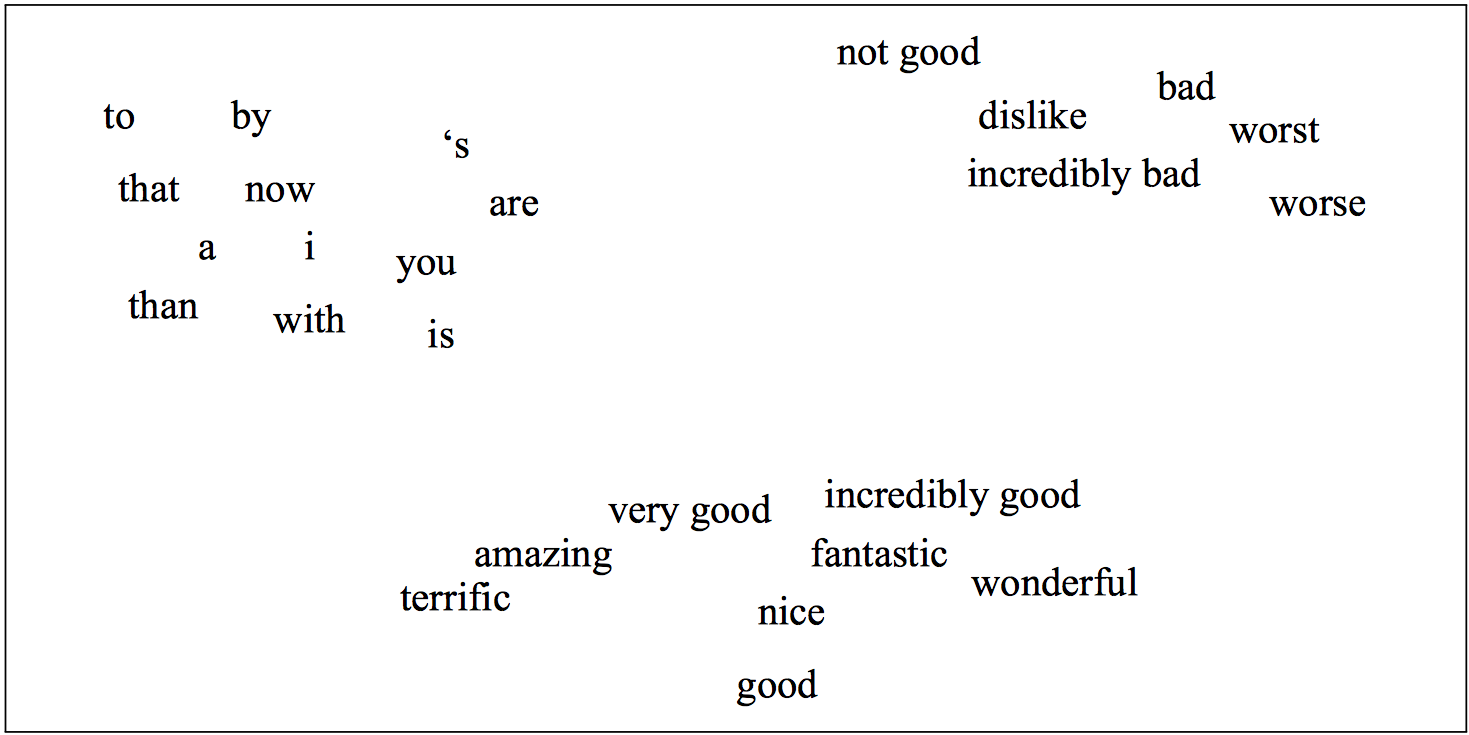
\includegraphics[width=\textwidth]{t_sne}
\caption{词向量降维后的可视化}
\label{fig:t_sne}
\end{figure}
%{\color{red}词嵌入降维图}\linkout{nlp_book}{107}

%{\color{red}词嵌入相关文献}\linkout{nlp_book}{128}

为实现这种从自然语言到向量空间的映射,自然语言处理发展历史上出现了许多理论和方法,例如Deerwester于1988年提出的潜在语义索引(Latent Semantic Indexing)方法\cite{LSI},以及该作者后续应用奇异值分解(SVD)对共现矩阵降维而实现的潜在语义分析方法(latent semantic analysis)\cite{LSA},在此后多年里被广泛应用于多种NLP任务,如认知模型\cite{cognitive_model},拼写检查\cite{spell_checking},写作评分\cite{essay_grading}等等。

随着近年来深度学习的发展,基于神经网络的自然语言模型开始流行,Bengio分别在2003年\cite{bengio2003}和2006年\cite{bengio2006}发表的成果表明,神经网络语言模型能在单词预测任务中出色地担任词嵌入转换的角色。

2013年,Mikolov提出了著名的连续词袋(CBOW)和Skip-gram模型\cite{skipgram},可以说这两种词嵌入模型的发明引发了NLP领域的深刻变革,至今为止这两种模型组成的Word2Vec方法仍被广泛使用于学术界和工业界。

%\begin{figure}[htp]
%\centering
%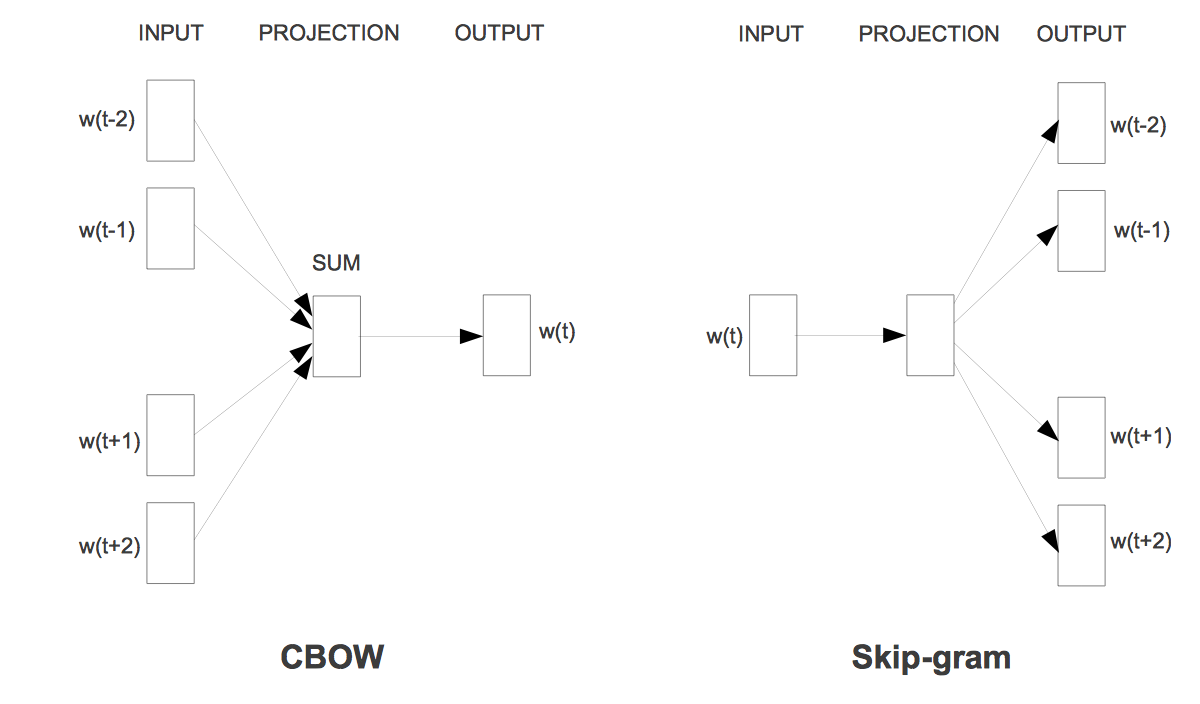
\includegraphics[width=\textwidth]{cbow_skipgram}
%\caption{Word2Vec的两种主要模型:CBOW与Skip-gram}
%\label{fig:cbow_skipgram}
%\end{figure}
%
%Word2Vec模型中,主要有Skip-Gram和CBOW两种模型,从直观上理解,Skip-Gram是给定中心词来预测上下文。而CBOW是给定上下文,来预测中心词。
%



\subsection{Skip-gram模型}
\subsection{子词模型}


%Word2Vec模型实际上分为了两个部分,第一部分为建立模型,第二部分是通过模型获取嵌入词向量。Word2Vec的整个建模过程实际上与自编码器(auto-encoder)的思想很相似,即先基于训练数据构建一个神经网络,当这个模型训练好以后,我们并不会用这个训练好的模型处理新的任务,我们真正需要的是这个模型通过训练数据所学得的参数,例如隐层的权重矩阵——后面我们将会看到这些权重在Word2Vec中实际上就是我们试图去学习的词向量。基于训练数据建模的过程,我们给它一个名字叫“Fake Task”,意味着建模并不是我们最终的目的。假如我们给定一个句子“The dog barked at the mailman”。
%


%\subsection{文件名、路径向量化}


\section{循环神经网络}
%简述RNN发展情况
\subsection{循环神经网络基本原理}

循环神经网络的主要用途是处理和预测序列数据。在全连接神经网络或卷积神经网络模型中,网络的结构都是从输入层到隐藏层再到输出层,层与层之间是全连接或者部分连接的,但每层之间的节点是无法连接的。而循环神经网络的隐藏层之间的节点是有连接的,隐藏层的输入不仅包括输入层的输出,还包括上一时刻隐藏层的输出。

\begin{figure}[htp]
\centering
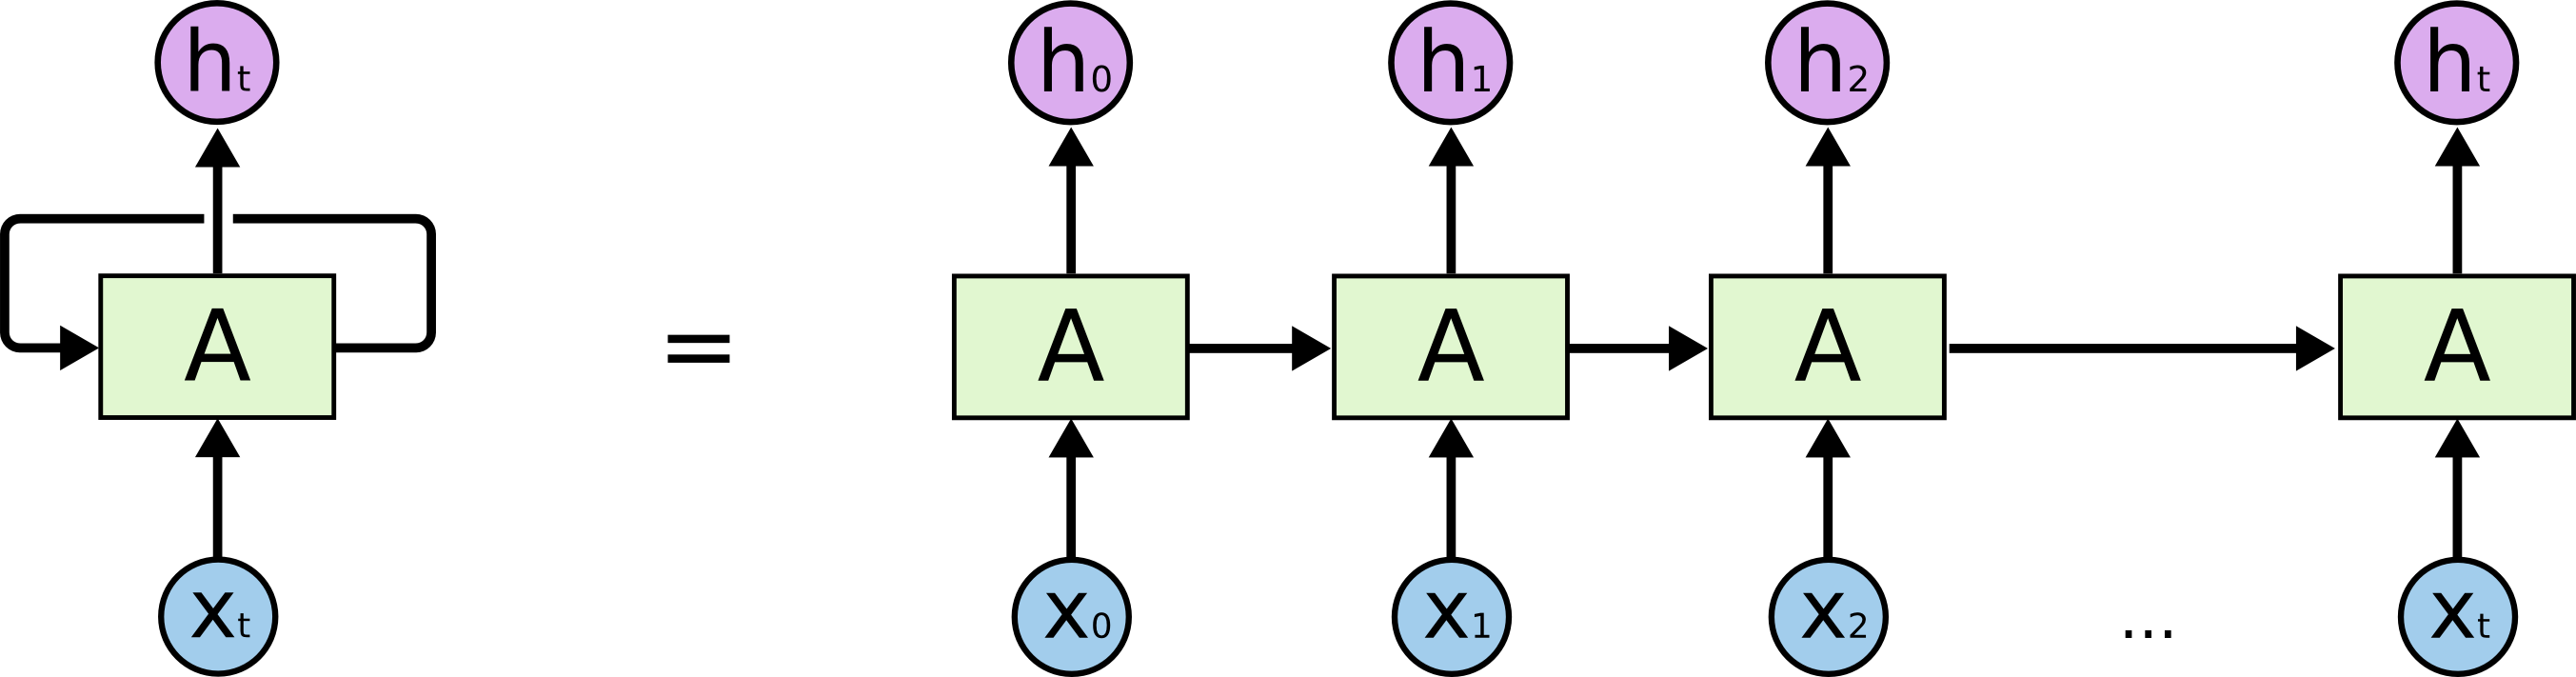
\includegraphics[width=\textwidth]{rnn_1}
\caption{RNN展开后的结构}
\label{fig:rnn_1}
\end{figure}
对于循环神经网络,一个非常重要的概念就是时刻。循环神经网络中每个时刻的输入都会对应一个输出。从图\ref{fig:rnn_1}中可以看到,循环神经网络的主体结构A的输入除了来自输入层$X_t$,还有一个循环的边来提供当前时刻的状态。在每一个时刻,循环神经网络的模块A会读取t时刻的输入$X_t$,并输出一个值$H_t$。同时A的状态会从当前步传递到下一步。因此,循环神经网络理论上可以被看作是同一神经网络结构被无限复制的结果。但出于优化的考虑,目前循环神经网络无法做到真正的无限循环,所以,现实中一般会将循环体展开。

\begin{figure}[htp]
\centering
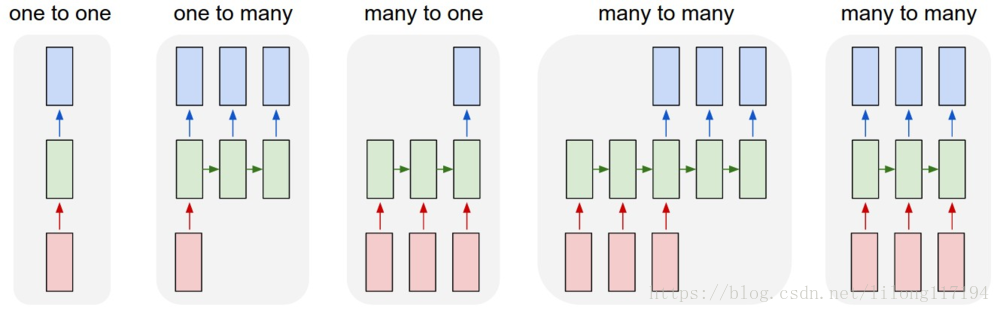
\includegraphics[width=\textwidth]{rnn_2}
\caption{RNN的多种模式}
\label{fig:rnn_2}
\end{figure}
RNN相对于传统的神经网络,它允许我们对向量序列进行操作:输入序列、输出序列、或大部分的输入输出序列。如图\ref{fig:rnn_2}所示,每一个矩形是一个向量,箭头则表示函数(比如矩阵相乘)。输入向量用红色标出,输出向量用蓝色标出,绿色的矩形是RNN的状态。RNN根据输入输出对应关系可分为如下几类:
\begin{enumerate}
    \item 没有使用RNN的Vanilla模型,从固定大小的输入得到固定大小输出(比如图像分类)
    \item 序列输出(比如图片字幕,输入一张图片输出一段文字序列)
    \item 序列输入(比如情感分析,输入一段文字然后将它分类成积极或者消极情感)
    \item 序列输入和序列输出(比如机器翻译:一个RNN读取一条英文语句然后将它以法语形式输出)
    \item 同步序列输入输出(比如视频分类,对视频中每一帧打标签)。
\end{enumerate}

\begin{figure}[htp]
\centering
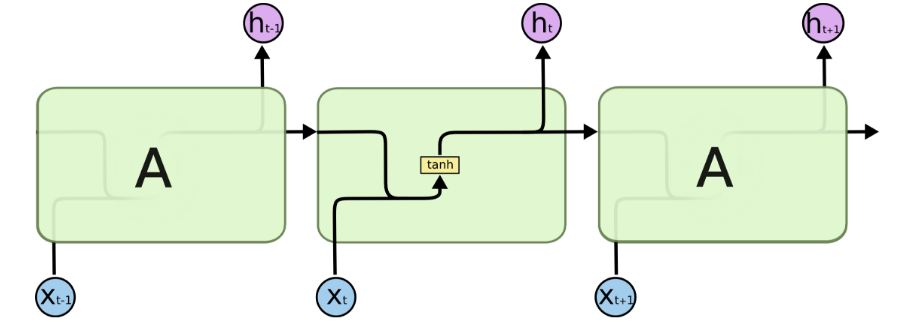
\includegraphics[width=\textwidth]{rnn_3}
\caption{使用单层全连接神经网络作为循环单元的RNN结构}
\label{fig:rnn_3}
\end{figure}

图\ref{fig:rnn_3}展示了一个使用最简单的循环体结构的循环神经网络,在这个循环体中只使用了一个类似全连接层的神经网络结构。下面将通过该图中所展示的神经网络来介绍循环神经网络前向传播的完整流程。

循环神经网络中的状态是通过一个向量来表示的,这个向量的维度也称为神经网络隐藏层的大小,设其为$h$。循环体中的神经网络的输入有两部分,一部分为上一时刻的状态$X_{t-1}$,另一部分为当前时刻的输入样本。对于时间序列数据来说,每一时刻的输入样例可以是当前时刻的数据;对于语言模型来说,输入样例可以是当前单词对应的词向量。
假设输入向量的维度为$x$,那么上图中循环体的全连接层神经网络的输入大小为$h+x$。也就是将上一时刻的状态与当前时刻的输入拼接成一个大的向量作为循环体中神经网络的输入。因为该神经网络的输出为当前时刻的状态,于是输出层的节点个数也为$h$(节点个数就是向量的维度,或者是隐藏层的大小),循环体中的参数个数为$(h+x)∗h+h(h+x)*h+h(h+x)∗h+h$个(这里可以理解为输入层有$h+x$个神经元,输出层有$h$个神经元,从而形成一个全连接的前馈神经网络,有$(h+x)*h$个权值,有$h$个偏置)。

同时循环体的神经网络输出不但提供给下一个时刻作为状态,同时还提供给当前的时刻作为输出。为了将当前时刻的状态转化为最终的输出,循环体还需要另外一个全连接神经网络来完成这个过程。这和卷积神经网络中最后的全连接层的意义是一样的。类似的,不同时刻用于输出的全连接神经网络中的参数也是共享的(参数一致)。

循环神经网络可以更好地利用传统神经网络结构所不能建模的信息,但同时,这也带来了更大的技术挑战——长期依赖(long-term dependencies)问题。因此,当前预测位置和相关信息之间的文本间隔就有可能变得很大。当这个间隔不断增大时,类似图\ref{fig:rnn_3}中给出的简单循环神经网络有可能丧失学习到距离如此远的信息的能力。或者在复杂语言场景中,有用信息的间隔有大有小、长短不一,循环神经网络的性能也会受到限制。

\subsection{长短期记忆与门控神经网络}

长短期记忆网络(long short term memory, LSTM)\cite{LSTM}的设计正是为了解决上述RNN的依赖问题,即为了解决RNN有时依赖的间隔短,有时依赖的间隔长的问题。其中循环神经网络被成功应用的关键就是LSTM。

\begin{figure}[htp]
\centering
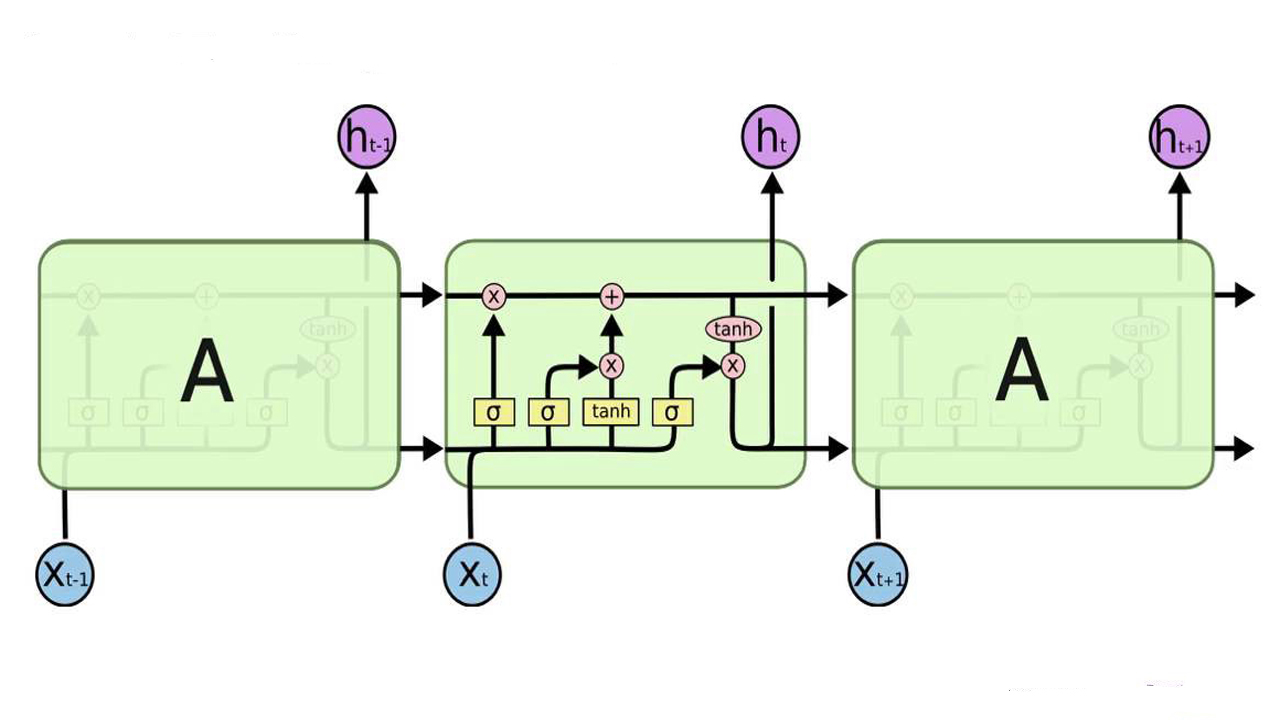
\includegraphics[width=\textwidth]{rnn_4}
\caption{长短期记忆网络LSTM}
\label{fig:rnn_4}
\end{figure}

LSTM的第一步是决定要从上一个时刻的状态中丢弃什么信息,其本质是由一个sigmoid全连接的前馈神经网络的输出管理,将这种操作称为遗忘门(forget get layer)。这个全连接的前馈神经网络的输入由向量$h_{t-1}$​和$x_t$组成,输出是$f_t$,1表示能够通过,0表示不能通过。
\begin{equation}
    f_t = \sigma(W_f \cdot [h_{t-1},x_t]+b_f)
\end{equation}

第二步决定哪些输入信息要保存到神经元的状态中。首先是一个sigmoid层的全连接前馈神经网络,称为输入门(input gate layer),其决定了哪些值将被更新;然后是一个tanh层的全连接前馈神经网络,其输出是一个向量$\tilde{C_t}$,该向量可以被添加到当前时刻的神经元状态中;最后根据两个神经网络的结果创建一个新的神经元状态。
\begin{align}
    i_t &= \sigma(W_i \cdot [h_{t-1,x_t}]+b_i) \\
    \tilde{C_t} &= \tanh(W_C \cdot [h_{t-1},x_t]+b_C)
\end{align}

第三步就可以上一时刻的状态$C_{t−1}$更新为当前状态$C_t$了。上述的第一步的遗忘门计算了一个控制向量,此时通过这个向量过滤一部分$C_{t-1}$状态;上述第二步的输入门根据输入向量计算了新状态,此时可以通过这个新状态$\tilde{C_{t-1}}$和$C_{t−1}$状态更新$C_t$
\begin{equation}
    C_t = f_t*C_{t-1} + i_t*\tilde{C_t}
\end{equation}
​	
最后一步就是决定神经元的隐状态$h_t$	,此时的输出根据上述第三步的状态$C_t$进行计算:首先通过sigmoid层生成一个过滤向量;然后通过一个$\tanh$函数计算当前时刻的$C_t$;最后通过sigmoid层输出当前时刻的输出。
\begin{align}
    o_t &= \sigma(W_o [h_{t-1},x_t]+b_o) \\
    h_t &= o_t * \tanh(C_t)
\end{align}

GRU(Gated Recurrent Unit)\cite{GRU}是长短时记忆网络单元的一个变种,其主要优点继承了LSTM能够解决长期依赖的特点,同时结构更简单,训练与推断的计算复杂度更低,目前已在自然语言处理和其他序列分析领域得到了广泛应用。
\begin{figure}[htp]
\centering
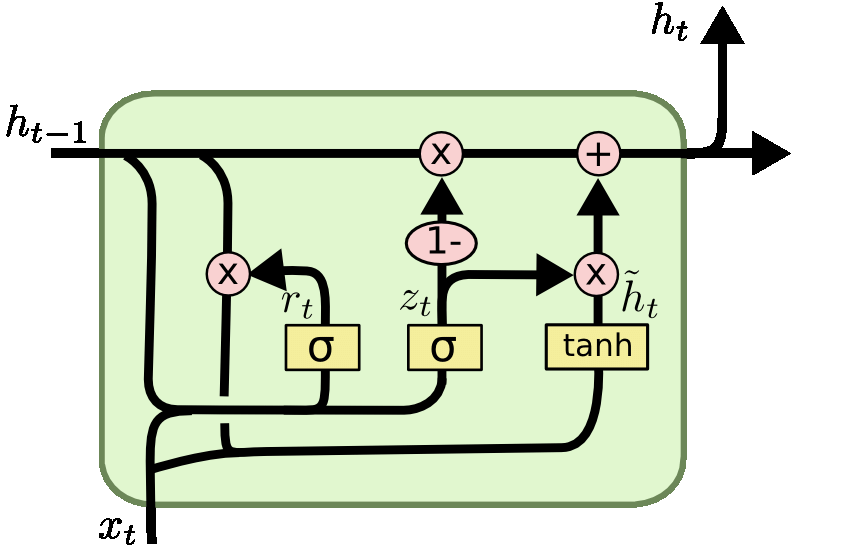
\includegraphics[width=\textwidth]{gru}
\caption{门控神经网络单元(GRU)}
\label{fig:gru}
\end{figure}





\section{本章小结}